
\documentclass[border=8pt, multi, tikz]{standalone} 
\usepackage{import}
\subimport{../layers/}{init}
\usetikzlibrary{positioning}
\usetikzlibrary{3d} %for including external image 

\def\ConvColor{rgb:yellow,5;red,2.5;white,5}
\def\ConvReluColor{rgb:yellow,5;red,5;white,5}
\def\PoolColor{rgb:red,1;black,0.3}
\def\UnpoolColor{rgb:blue,2;green,1;black,0.3}
\def\FcColor{rgb:blue,5;red,2.5;white,5}
\def\FcReluColor{rgb:blue,5;red,5;white,4}
\def\SoftmaxColor{rgb:magenta,5;black,7}   

\newcommand{\copymidarrow}{\tikz \draw[-Stealth,line width=0.8mm,draw={rgb:blue,4;red,1;green,1;black,3}] (-0.3,0) -- ++(0.3,0);}

\begin{document}
\begin{tikzpicture}
\tikzstyle{connection}=[ultra thick,every node/.style={sloped,allow upside down},draw=\edgecolor,opacity=0.7]
\tikzstyle{copyconnection}=[ultra thick,every node/.style={sloped,allow upside down},draw={rgb:blue,4;red,1;green,1;black,3},opacity=0.7]

\node[canvas is zy plane at x=0] (temp) at (-3,0,0) {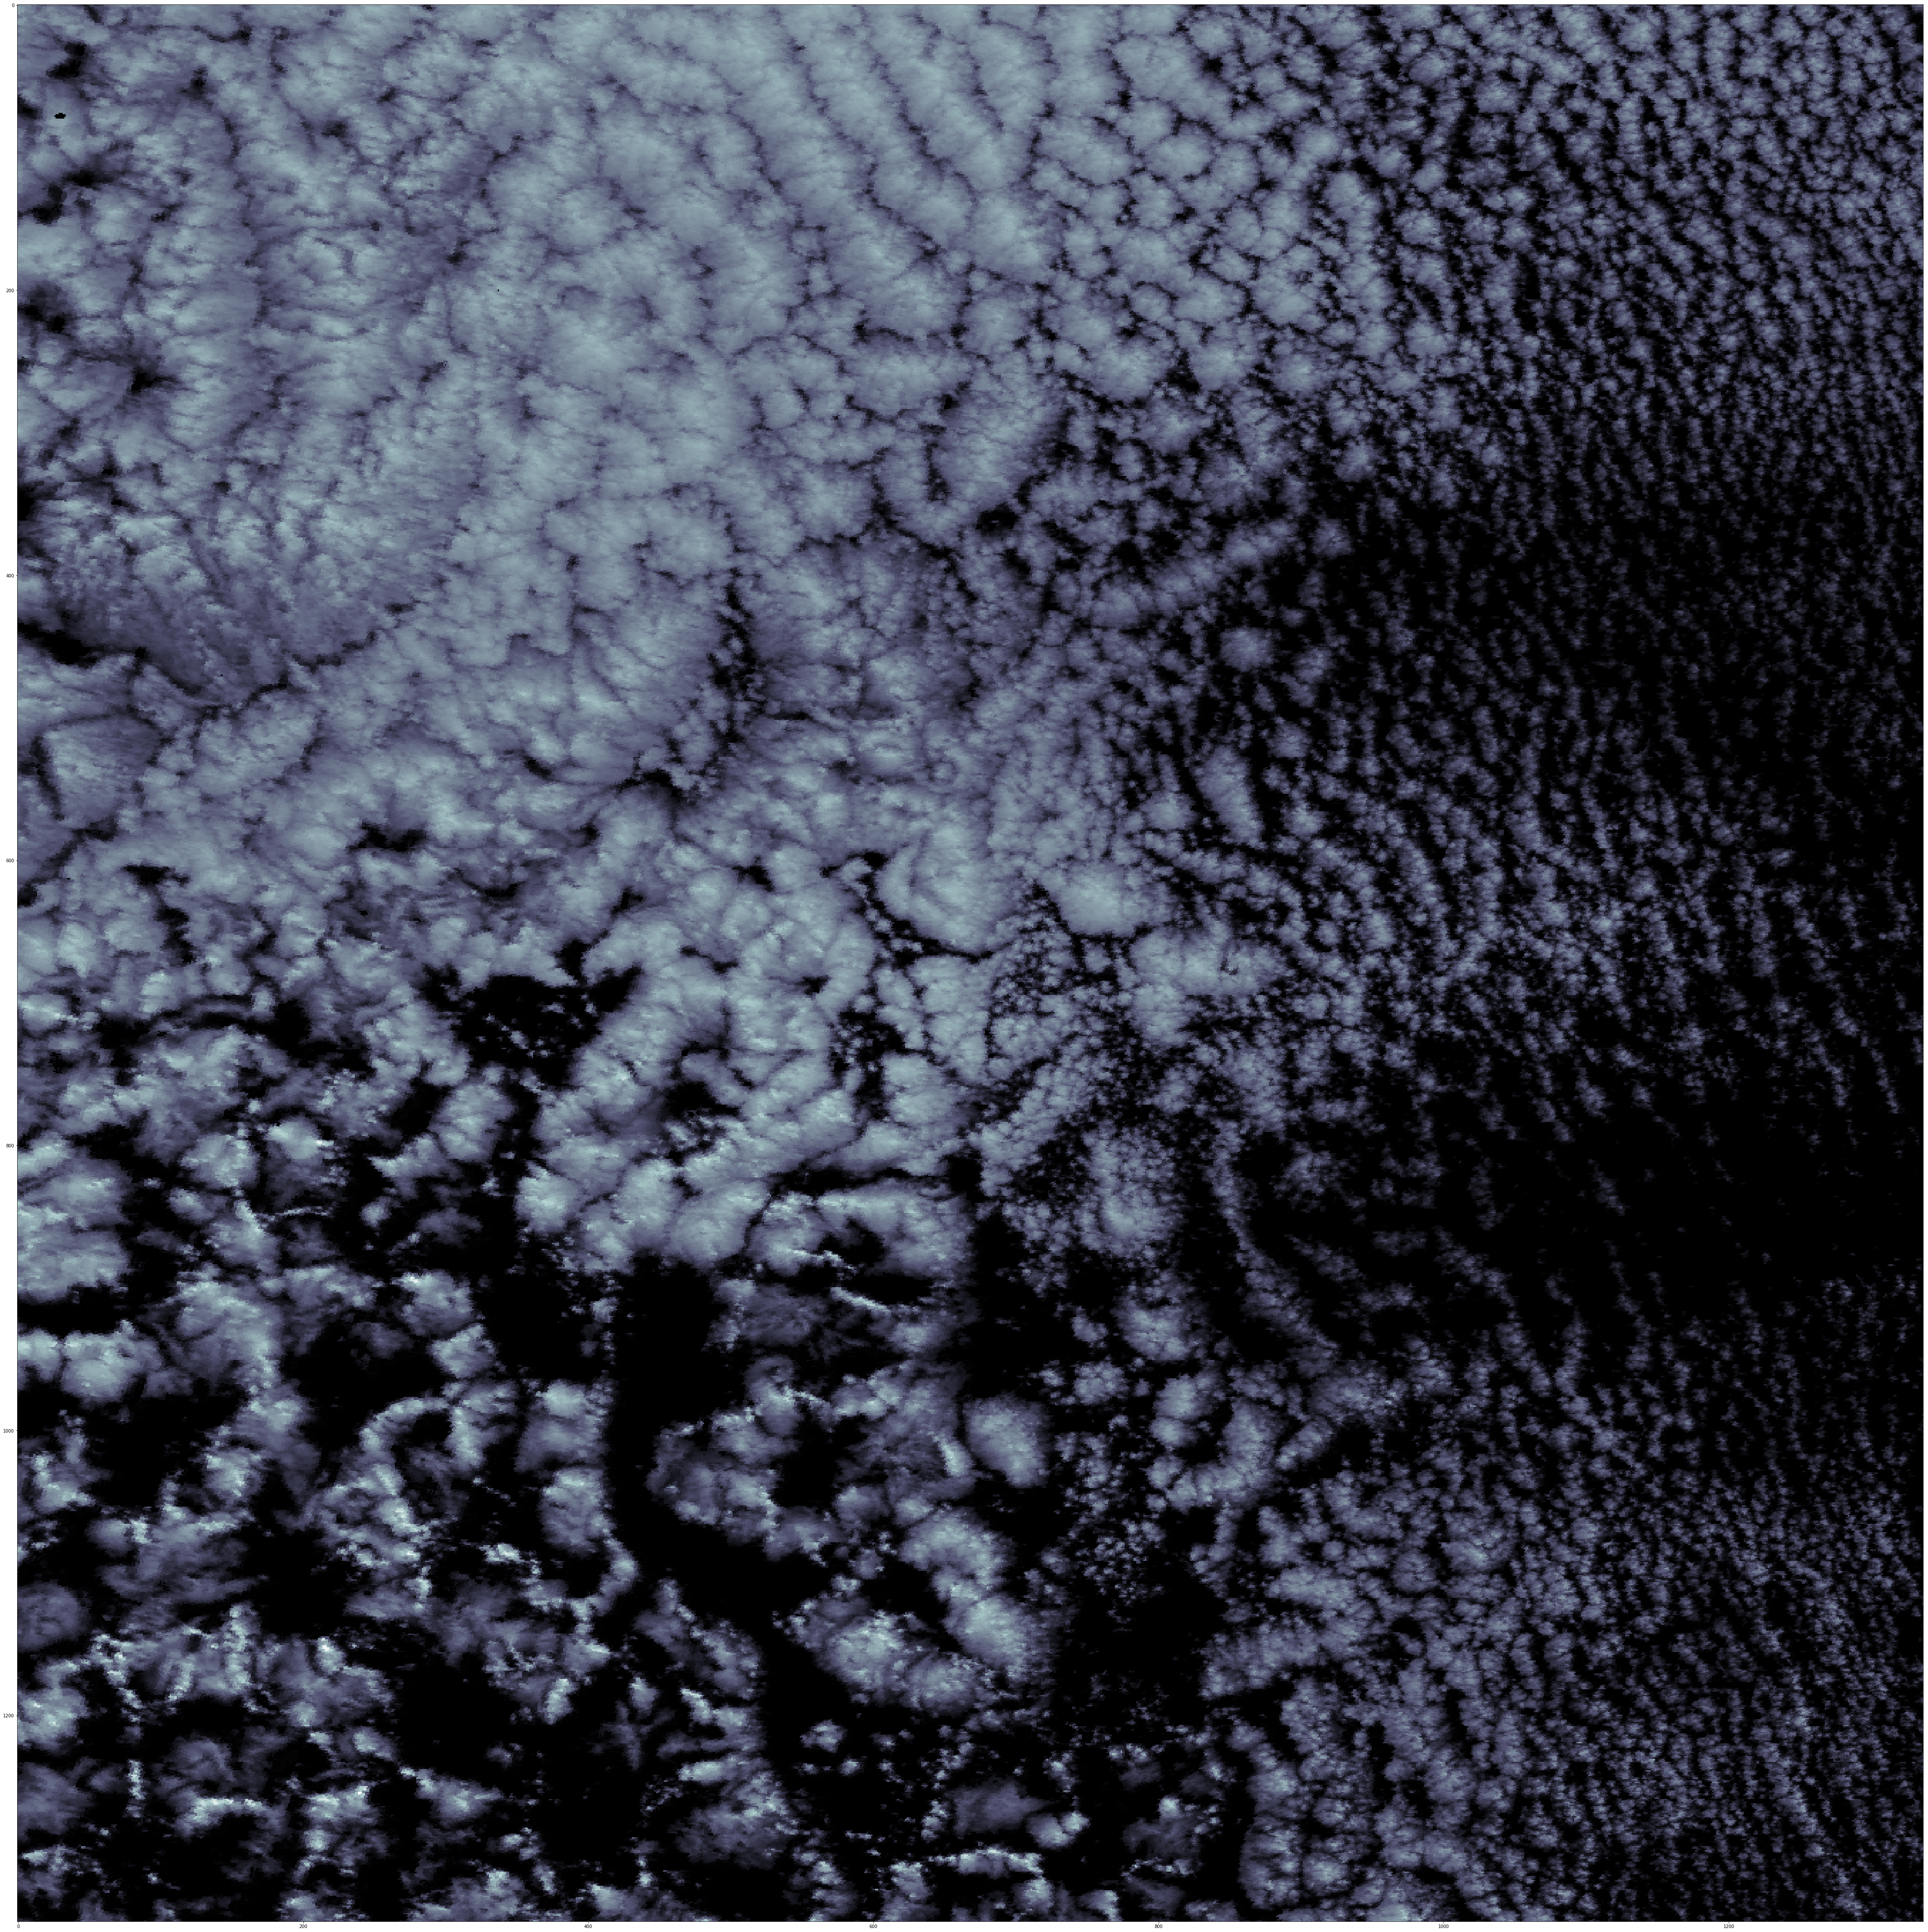
\includegraphics[width=8cm,height=8cm]{./coast_of_chile_high_res.png}};

\pic[shift={(0,0,0)}] at (0,0,0) 
    {Box={
        name=conv_b01_l01,
        caption= ,
        xlabel={{16, }},
        zlabel=128,
        fill=\ConvColor,
        height=40.0,
        width=5.0,
        depth=40.0
        }
    };

\pic[shift={(0,0,0)}] at (conv_b01_l01-east) 
    {Box={
        name=relu_b01_l01,
        caption= ,
        xlabel={{16, }},
        zlabel=128,
        fill=\ConvColor,
        height=40.0,
        width=5.0,
        depth=40.0
        }
    };

\end{tikzpicture}
\end{document}
